\documentclass[utf8,xcolor=table]{beamer}

\usepackage{cmap}
\usepackage[T2A]{fontenc}
\usepackage[utf8]{inputenc}
\usepackage[english,russian]{babel}
%\usepackage{tikz-uml}
\usepackage{minted}

\mode<presentation>{
	\usetheme{CambridgeUS}
}

\renewcommand{\t}[1]{\ifmmode{\mathtt{#1}}\else{\texttt{#1}}\fi}

\title{Редактор схем с распознаванием}
\author{Егор Суворов}
\institute[CSCenter]{Практика, осень 2014 -- весна 2015\\Куратор: Евгений Линский}
\date[21.05.2015]{Четверг, 21 мая 2015 года}

\setlength{\arrayrulewidth}{1pt}

\begin{document}

\begin{frame}
\titlepage
\end{frame}

\begin{frame}[t]{Постановка задачи}
  Мотивация: оцифровка рисуемых схем в процессе рисования,
  чтобы был сразу виден результат.

  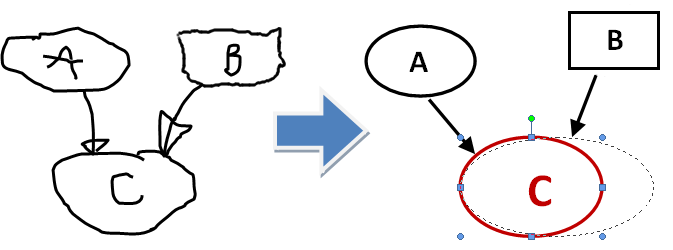
\includegraphics[width=\textwidth]{problem}
  \begin{itemize}
  \item~<<Умное перо>> для рисования векторных схем
  \item Распознавание фигур, соединений, жестов
  \item Автоматическая структуризация схемы
  \item Экспорт в SVG
  \end{itemize}
\end{frame}

\begin{frame}[t]{Результаты первого семестра}
  \begin{columns}[T]
  \begin{column}{.6\textwidth}
    \begin{itemize}
    \item Распознавание:
      \begin{itemize}
      \item Прямоугольник, эллипс, отрезок
      \item Жесты удаления и перетаскивания
      \item Соединение фигур
      \end{itemize}
    \item Экспорт в SVG
    \item Real-time результат распознавания
    \item Undo
    \end{itemize}
  \end{column}
  \begin{column}{.4\textwidth}
    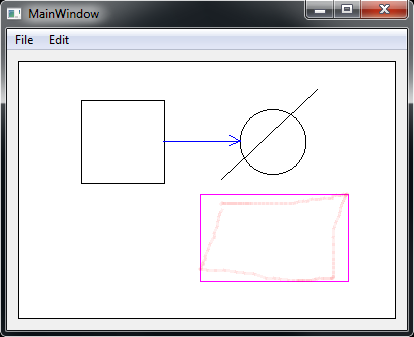
\includegraphics[height=3.5cm]{demo_scr}
  \end{column}
  \end{columns}
  \begin{itemize}
  \item Технические детали:
    \begin{itemize}
    \item Написано на C++11 и Qt, работает на Windows/Linux
    \item Написаны unit-тесты на геометрические вычисления
    \end{itemize}
  \end{itemize}
\end{frame}

\begin{frame}[t]{Обзор изменений за второй семестр}
  \begin{itemize}
  \item Порт на Android
  \item Распознавание ломаных и их сглаживание
  \item Текст на фигурах и отрезках (unicode, многострочный)
  \item Симметризация фигур и выравнивание фигур в дерево по запросу
  \item Юнит-тесты для распознавания, ввода-вывода; стресс-тесты
  \end{itemize}
  \begin{center}
    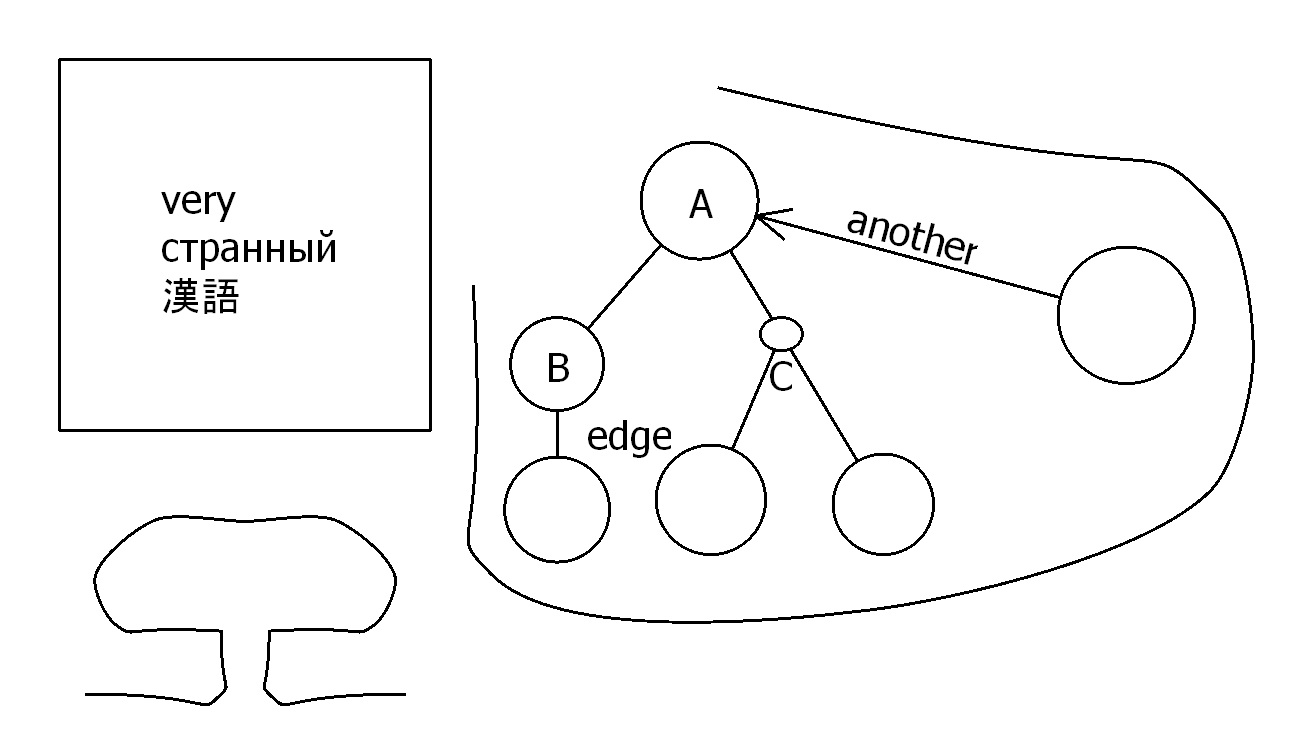
\includegraphics[height=4cm]{demo}
  \end{center}
\end{frame}

\begin{frame}[t]{Обзор улучшений распознавания}
  \begin{itemize}
  \item На desktop учитывается скорость пера (остановках пера считается <<углом>> фигуры)
  \item Добавлена поддержка ломаных
    \begin{itemize}
      \item Можно ставить стрелки на сегментах ломаных
      \item Ломаные обрабатываются алгоритмом Рамера-Дугласа-Пекера для уменьшения количества точек
      \item Отрезки ломаных между <<углами>> сглаживаются кривыми Безье
    \end{itemize}
  \item Введена защита от случайных касаний на touch-устройствах
  \end{itemize}
\end{frame}

\begin{frame}[t]{Описание алгоритма распознавания}
  \begin{itemize}
  \item Короткие движения "--- клики: выделение фигур или добавление/удаление стрелок
  \item Быстрое <<зачёркивающее>> движение "--- удаление фигуры
  \item Путь от одной фигуры к другой "--- соединение
  \item Путь от границы выделенной фигуры "--- перенос
  \item Кандидаты из регулярных фигур:
    \begin{center}
      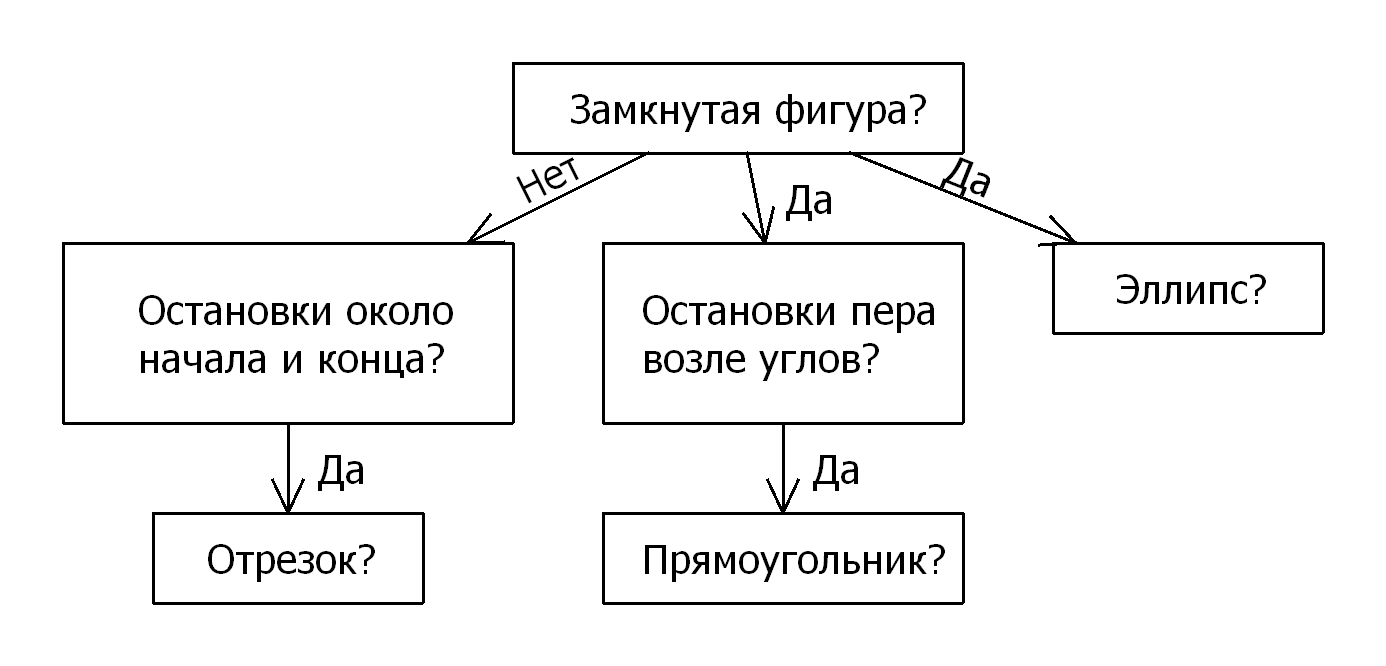
\includegraphics[height=2.5cm]{algo_cand}
    \end{center}
  \item Если движение сильно отличается от контуров кандидатов, рисуем кривую
  \end{itemize}
\end{frame}

\begin{frame}[t]{Симметризация ломаных}
  Можно выбрать произвольную ломаную и сделать её вертикально/горизонтально симметричной.
  \begin{center}
    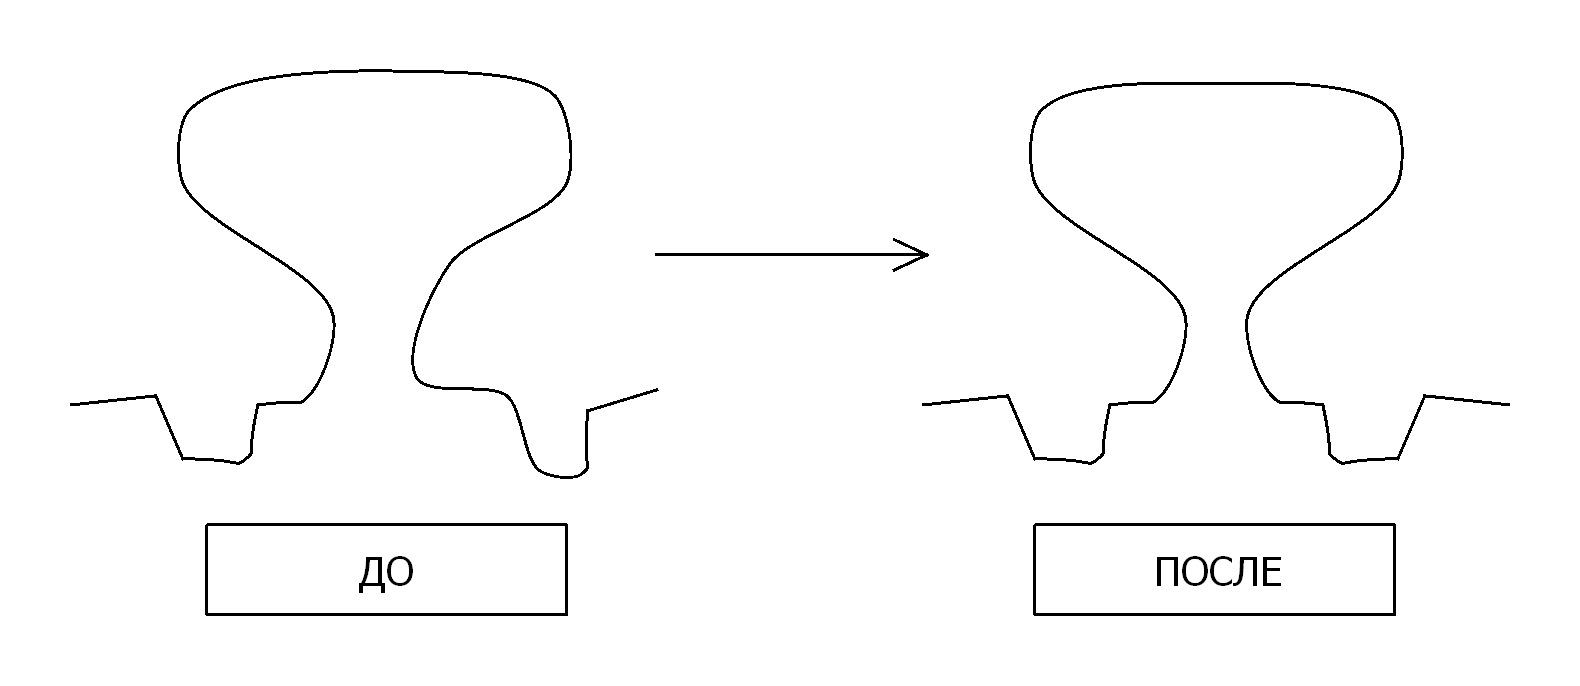
\includegraphics[height=4cm]{demo_symm}
  \end{center}
  Выбирается кусок ломаной до линии симметрии и отражается.
\end{frame}

\begin{frame}[t]{Выравнивание дерева}
  Можно выбрать <<вершину>> (эллипс или прямоугольник) и попросить упорядочить детей в виде дерева.

  \begin{center}
  \begin{tabular}{cc}
    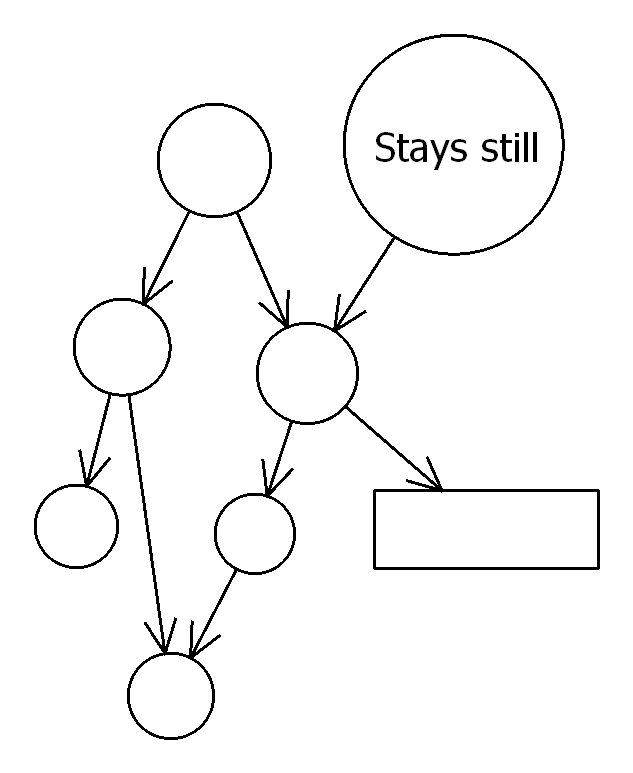
\includegraphics[scale=0.2]{demo_tree_1}
    &
    \raisebox{1cm}{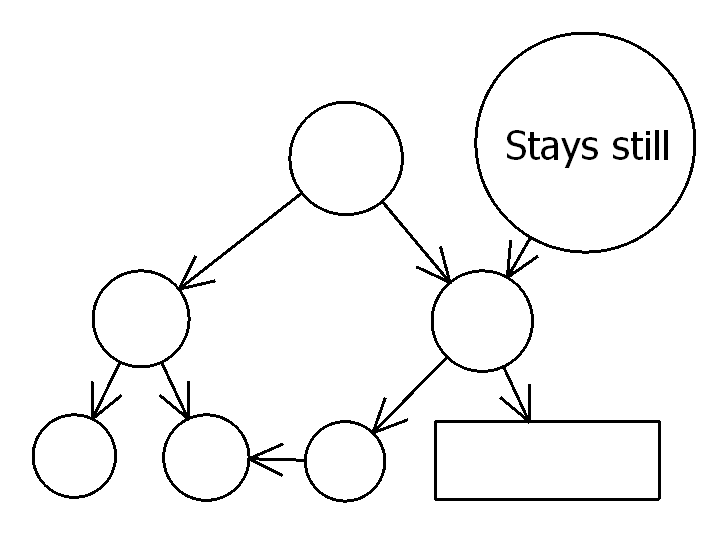
\includegraphics[scale=0.2]{demo_tree_2}}
    \\
    До
    &
    После
  \end{tabular}
  \end{center}

  BFS'ом обходятся достижимые вершины, строится дерево обхода, после чего поддеревья рекурсивно упорядочиваются.
\end{frame}

\begin{frame}[t]{Прочие улучшения интерфейса}
  \begin{itemize}
  \item Выравнивание элементов по сетке
  \item Можно менять масштаб и прокручивать окно при редактировании. Изначальный масштаб подстраивается под DPI экрана
  \item На фигуры можно добавлять текст
    \begin{itemize}
    \item Автоматически располагается либо вне фигуры, либо внутри "--- где хватает места
    \item На отрезках наклоняется вместе с отрезком
    \item Можно делать многострочным, поддерживается Unicode
    \end{itemize}
  \item Все возможности сохраняются при экспорте в PNG
  \item При экспорте в SVG сохраняется всё, кроме сглаживания ломаных.
  \end{itemize}
\end{frame}

\begin{frame}[t]{Автоматические тесты}
  \begin{itemize}
  \item Ввод-вывод заранее подготовленной модели
  \item Стресс-тестирование
    \begin{itemize}
    \item Случайные модификации модели
    \item Проверка корректности ввода-вывода
    \item Проверка отсутствия утечек памяти и некорректных ссылок
    \end{itemize}
  \item Тестирование распознавания: подготовлено 57 ручных треков, для каждого известен необходимый результат распознавания (тип фигуры)
  \end{itemize}
\end{frame}

\begin{frame}[t]{Скриншот}
  \begin{center}
    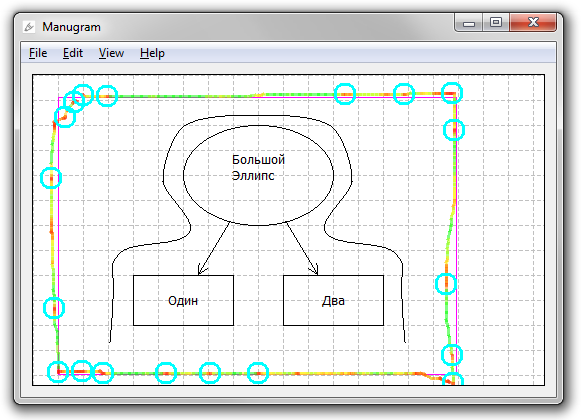
\includegraphics[scale=0.5]{demo_scr2}
  \end{center}
\end{frame}

\begin{frame}[t]{Ссылки}
  \begin{itemize}
  \item \href{mailto:egor_suvorov@mail.ru}{\t{egor\_suvorov@mail.ru}}
  \item \href{http://github.com/cscenter/manugram/}{\t{github.com/cscenter/manugram}}
  \end{itemize}
\end{frame}

\end{document}
